\chapter{Sequencing to explore mechanism}

\section{Therapeutics}
 
\subsection{Antibiotics}

While NGS has great promise for infectious disease diagnostics, therapies are required to eradicate infections once identified. In the late 19\text{th} century, pathogen-immune serum was used as a successful treatment against infectious agents. This approach encouraged scientists to develop chemicals that kill the specific pathogens, starting with Ehrlich\'s "magic bullet" against syphilis (arsphenamine) in 1910. Within two decades, a generation of scientists were working on antibiotics. As a result of these efforts, sulfa drugs were developed in 1936 and penicillin in 1943. Nearly all antibiotics in use today are compounds that were discovered during the 1940s to 1960s - the golden era of antibiotic discovery - or their derivatives. Most of these compounds were discovered by screening soil-derived actinomycetes, but natural product discovery became impractical due to the increasing difficulty of identifying new classes of antibiotics against the background of known compounds \cite{Lewis:2013bp}.

\subsection{Antivirals}

When antiviral drugs were first developed in the 1960s, they did not seem to be particularly promising, with a few exceptions. In response to the HIV/AIDS pandemic, however, the development of antiretroviral drugs markedly expanded the arsenal of available antiviral agents. By the mid 2000s, 37 chemicals (plus IFN- $\alpha$ in both pegylated and unpegylated forms) were formally approved for the treatment of viral infection \cite{Clercq:2004ba}. At least half of these were intended to treat HIV infections and there are a similar number of compounds are under preclinical or clinical development, at least half of which were expected to reach the antiviral drug market.

Critically, these drugs largely target molecules required for viral replication. Antiviral strategies generally target viral DNA polymerase for the treatment of DNA virus infections, helicase/NTPase for the treatment of HSV, HCV, or SARS-CoV infections, IMP dehydrogenase for the treatment of HCV and some negative-strand RNA virus (for example, arena- and bunyavirus) infections, SAH hydrolase for the treatment of other negative-strand RNA virus infections such as Ebola and Marburg virus or RNA virus infections such as rotavirus, and RNA-dependent RNA polymerase for the treatment of other positive-strand RNA virus (e.g., flavivirus) infections \cite{Clercq:2004ba}.

\subsection{The challenge}

A central challenge in the fight against infectious disease is evolution: pathogens mutate in response to selective pressure imposed by treatment, resulting in an escalating arms-race between man and infection. Consider that RNA viruses exhibit extremely high mutation rates, orders of magnitude greater than those of most DNA-based life forms. Studies carried out to date suggest that many RNA viruses generate $10^{-4}$ to $10^{-6}$ errors per nucleotide, which is equivalent to approximately one mutation per genome per replication cycle \cite{Lauring:2013iq}. Given the large population sizes observed in both experimental and natural infections with these viruses, every possible point mutation and many double-mutation combinations could theoretically be generated during each replication cycle within a population.

\section{Mechanism}

\subsection{The case for mechanistic studies}

Considering that pathogens evolve, the effectiveness of therapies today cannot be assured tomorrow. Indeed, there are now great concerns about the emergence of antibiotic resistant bacteria as well as viral strains (e.g., of HIV) that no longer respond to antivirals. In turn, there are been great emphasis on understanding the molecular principles that underlie infectious disease  \cite{Fox:2014fj}. These molecular principles can be used to devise new therapeutic strategies. 

\subsection{The importance of molecular interactions}

The study molecular interactions, particularly in the case of viruses, has been a productive way to devise new therapeutic strategies. This is particularly evident in the case of Hepatitis C Virus (HCV), a global health concern with 2 - 3\% of the world?s population infected \cite{Wilson:2014ba}. HCV is a positive-sense single-stranded RNA virus of the family Flaviviridae. The 9.6 kb genome contains a single open reading frame that is subsequently cleaved into 10 viral proteins and is flanked by UTRs. 

The standard of care against HCV is a combination IFN / ribavirin, although many patients do not benefit from this treatment. With this in mind, is widely expected that in future small molecule drugs that target specific viral proteins that play essential roles in the viral life cycle (a.k.a. direct-acting antivirals) will replace IFN-based therapies. The approvals of two protease inhibitors (2011) and polymerase inhibitors (2013) were significant milestones in this regard.

Parallel efforts to discover novel viral targets have also been effective. For example, HCV interacts with numerous micro-RNAs (miRNAs), which are molecules predicted to regulate at least 60\% of all human genes. One miRNA, miR-122, promotes HCV accumulation through direct interactions with the viral genomic RNA. Mechanistci studies have shown that miR-122 stabilizes the viral RNA by protecting the 5\'  terminus from degradation by the host exonuclease, Xrn-1 \cite{Wilson:2014ba}.

With this molecular knowledge in mind, agents that target miR-122 have been used to treat HCV infection. In a recent Phase II clinical trial, miravirsen, an antisense locked nucleic acid molecule that binds to and sequesters miR-122, reduced serum HCV titers in treatment HCV-infected patients. At the highest doses used, HCV RNA became undetectable, but rebounded following completion of the 4-week course of miravirsen mono-therapy. A 12-week course of treatment is currently being tested to determine if patients can achieve sustained viral clearance \cite{Wilson:2014ba}.

Targeting host molecules, such as miR-122, may have numerous potential advantages, including a higher barrier to resistance, pan-genotypic activity and a wide range of druggable targets (whereas viral targets are limiting) \cite{Wilson:2014ba}. Thus, a better understanding of the host-viral interaction networks that underlie translation and replication are likely to reveal novel targets for therapeutic intervention.

\section{RNA-protein interactions}

Considering the importance of molecular interaction networks for the development of new therapeutic strategies, we ask whether NGS-based strategies may be used to better understand infectious disease mechanism. Because HCV is a very well-studied model system, we first considered how NGS may be used to better understand RNA-viruses. Two points were clear: (1) RNA-protein interactions are central for the translation and replication of RNA viruses, with host proteins (e.g., ribosomes) critical for the production of viral products. (2) New NGS-based biochemical methods, such as CLIP-seq, make it possible to perform genome-wide RNA-protein measurements \cite{Konig:2012ww}. With these points in mind, we decided to build a computational pipeline for processing CLIP-seq data that can be easily applied to viruses. 
 
\section{CLIP pipeline}

\subsection{Philosophy}

Considering the diverse reach of RNA-binding proteins (RBPs) in cell biology, substantial effort has been focused on methods for genome-wide interrogation of RNA protein interactions using NGS. By stabilizing direct interactions in vivo combined with stringent purification steps, UV cross-linking immunoprecipitation and sequencing (CLIP-seq) enables specific isolation of an RBP\'s RNA-binding sites for NGS \cite{Konig:2012ww}.

\begin{figure*}
\center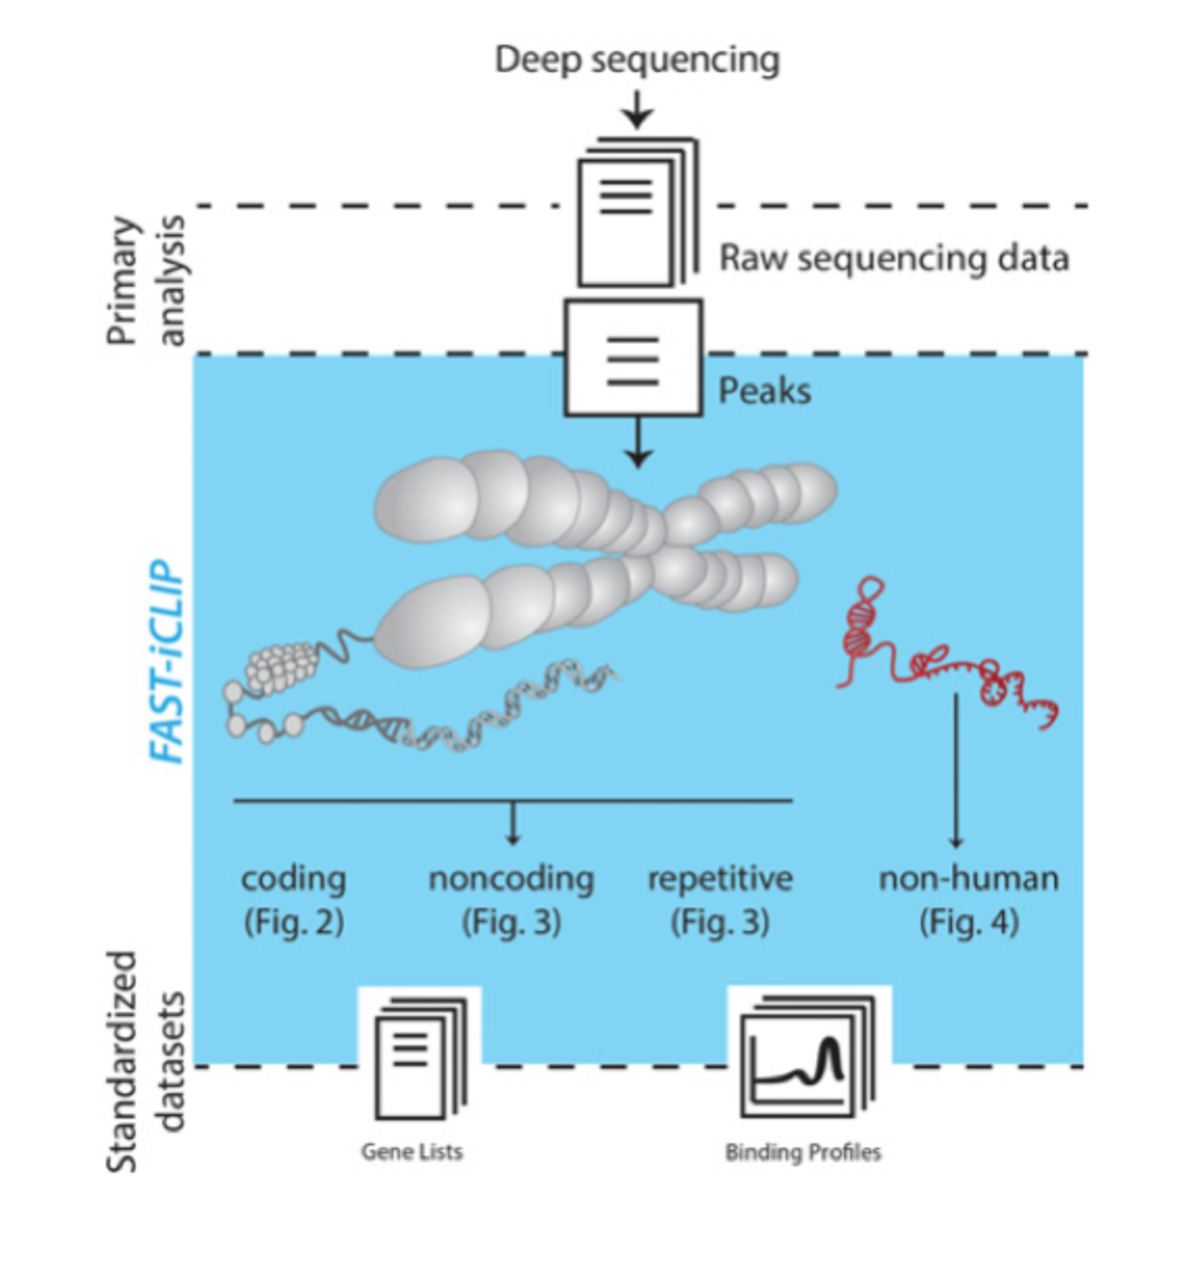
\includegraphics[width=120mm,scale=0.5]{Figures/Fig15}
\caption{CLIP analysis workflow.}
\label{fig:Fig15}
\end{figure*}

Much of the pioneering work has been focused on well-studied proteins and the protein-coding transcriptome, leading to numerous important advances on both methodological (PAR-CLIP, iCLIP, and BrdU-CLIP) and computational fronts \cite{Flynn:2014bi}. These results have spurred broader interest in CLIP, particularly with respect to the interactomes of noncoding RNAs or diversity of viruses and microbes that impinge on human health \cite{Consortium:2012bb}. While RNA protein complexes such as the ribosome and spliceosome are well-studied, a vast and enigmatic repertoire of noncoding and nonhuman RNA-protein interactomes await further characterization. 

Yet, extending CLIP across many RBPs is challenging for at least two reasons: (1) The sample preparation protocol is inefficient and time consuming and (2) informatic methods are not easily implemented or generally applicable to any RBP, particularly if RBP targets are not obvious \emph{a priori}. To put these challenges in context, the CLIP workflow can be thought of as a stack of tasks - starting with NGS biochemistry, followed by informatic transformations of the resulting data, and finally protein-specific questions or analyses. Because the specificity of work increases as one moves across the stack, we sought to address common challenges to any CLIP investigation by improving the efficiency of sample preparation, extending the intermediate analysis to include a diverse set of user-definable transcriptomes (protein coding, non-coding, non-human, etc), and also standardizing data format output such that comparisons between RBPs are straightforward (Figure ~\ref{fig:Fig15}).

\section{CLIP pipeline applications}

Prior to testing our pipeline on non-human genomes, we first tested it on human targets. We focused on RNA helicases, which are conserved enzymes that use the energy of ATP to remodel RNA secondary structures and RNA-protein complexes. 

\subsection{Application to DDX21}

The nucleolar helicase DDX21 is required for ribosome biogenesis and pre-rRNA processing, but the specific mechanism underlying this critical role remains unknown. To explore this, ChIP-seq in HEK293 cells was first performed, revealing DDX21-binding at promoters for genes involved in the ribosomal pathway. DDX21 knockdown decreased the steady-state levels of transcripts originating from DDX21-bound promoters, indicating that DDX21 associates with and positively regulates transcription of Pol I- and Pol II-dependent ribosomal genes \cite{Calo:2014ix}.

The next question was whether DDX21 associates with RNAs directly involved in pre-rRNA processing. There were two clear candidates: (1) rRNA may be bound by DDX21. rRNA must be both cleaved and processed with chemical medications, such as pseudouridylation. These chemical modifications aid in the formation of ribosome complexes and may aid translational efficiency. (2) Chemical modifications to rRNA are made - in part - by snoRNAs, a specific class of small non-coding RNAs that guide protein complexes (e.g., enzymes) to specific modification sites on rRNA. 

Our CLIP pipeline was well-suited to this question, because it was designed to analyze non-coding RNAs, including both rRNA and snoRNAs. In turn, we performed tandem purification iCLIP and processed the data, which partitions the data by non-coding RNA category. We found that DDX21 interacts with a diverse set of RNAs, of which rRNA and snoRNAs were most highly represented (Figure ~\ref{fig:Fig16}).

\begin{figure*}
\center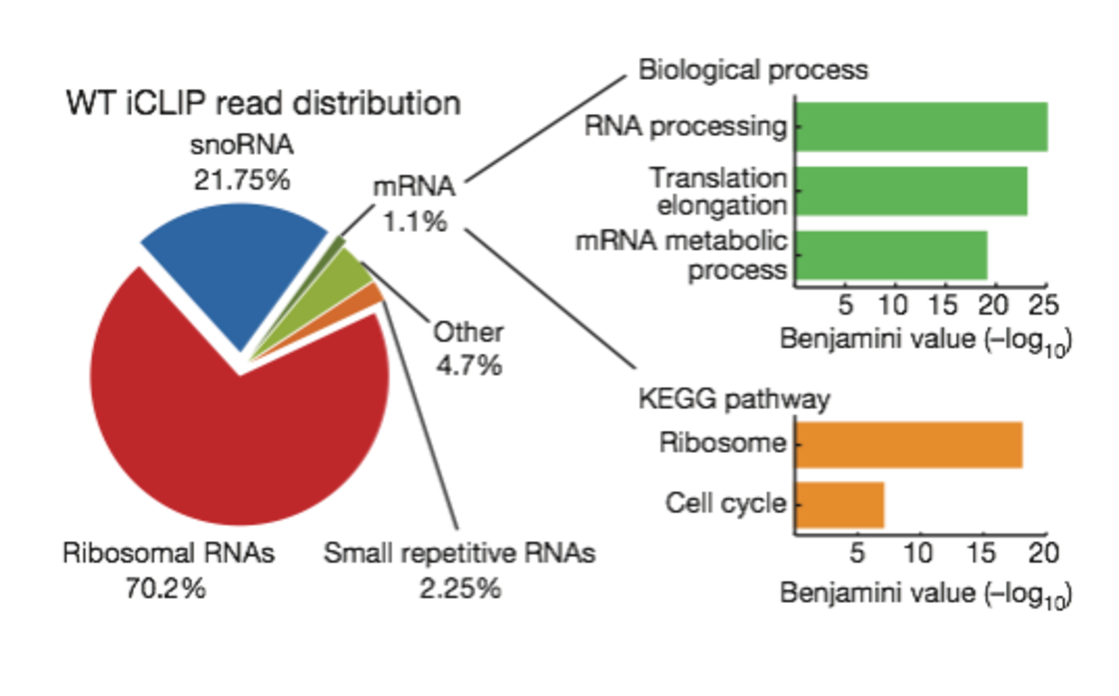
\includegraphics[width=120mm,scale=0.5]{Figures/Fig16}
\caption{Bound classes of RNAs to DDX21.}
\label{fig:Fig16}
\end{figure*}

For the mRNAs bound, Gene ontology term and KEGG pathway analysis linked these mRNAs to ribosome function. This provides some evidence that the bound targets are bone-fide, rather than noise, as their is functional consistency between these genes and the predicted target pathway of DDX21. However, this is not enough. There are at least two ways additional ways to validate the results: (1) In order to convince ourselves that the CLIP signal is not spurious or noise, we can ask whether the observed binding profile is unique to DDX21 relative to other CLIPed proteins. (2) Most importantly, we can perform functional studies based upon, and to validate, the hypotheses generated by the CLIP data.

\begin{figure*}
\center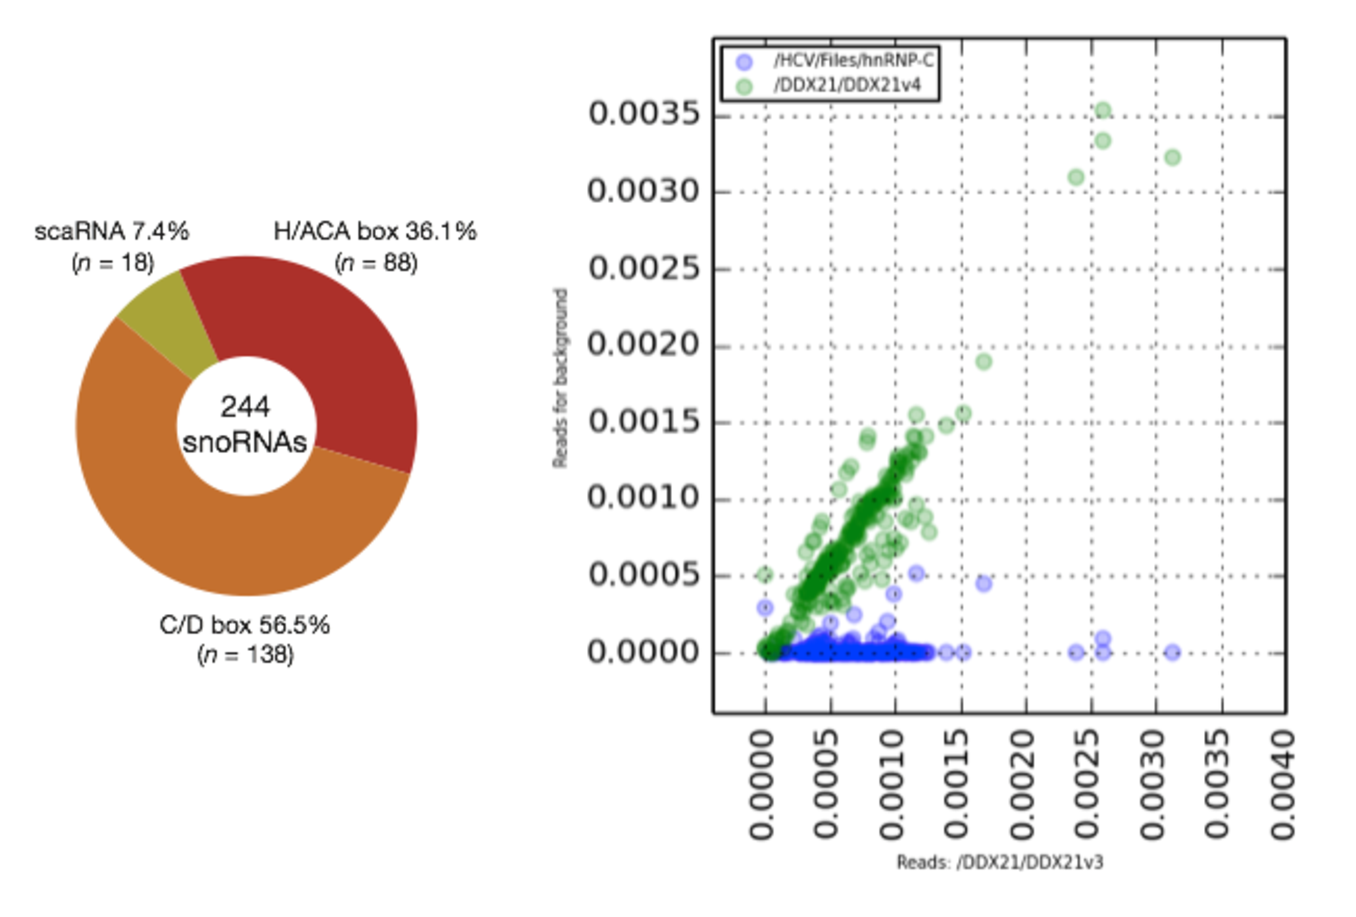
\includegraphics[width=120mm,scale=0.5]{Figures/Fig17}
\caption{The snoRNA binding profile of DDX21.}
\label{fig:Fig17}
\end{figure*}

Because the CLIP pipeline generates a consistent data format for each protein processed, it is relatively easy to compare results for any class of non-coding RNA. We would like to compare the number of reads mapping to a particular transcript between experiments. Of course, experiments have different degrees of sequencing depth. To correct for this, we can divide the number of hits to a particular gene by the total number of mapped reads, resulting in a normalized count ratio that is more reasonable to compare. We perform this comparison for each bound snoRNA gene between the DDX21 CLIP dataset and hnRNPC, another RNA-binding protein on which iCLIP was performed \cite{Zarnack:2013iv} (Figure ~\ref{fig:Fig17}).

A scatter plots of normalized counts comparing DDX21 replicates along with DDX21 and hnRNPC indicates two key points: First, snoRNAs are similarly bound in DDX21 replicates. Second, these same snoRNAs are not also bound by hnRNPC. In turn, the snoRNA binding patters appears to be both reproducible as well as specific to DDX21. Yet, this is not sufficient to make strong claims about function. Using immunoprecipitation, we found that DDX21 cross-links to NOP58, fibrillarin and dyskerin, which are all protein components of snoRNP complexes. These data place DDX21 within snoRNAP complexes. These complexes perform enzymatic modification of rRNA, which suggests a testable hypothesis: if DDX21 is a key element of the snoRNP, then DDX21 knock-down should inhibit rRNA modification.

\begin{figure*}
\center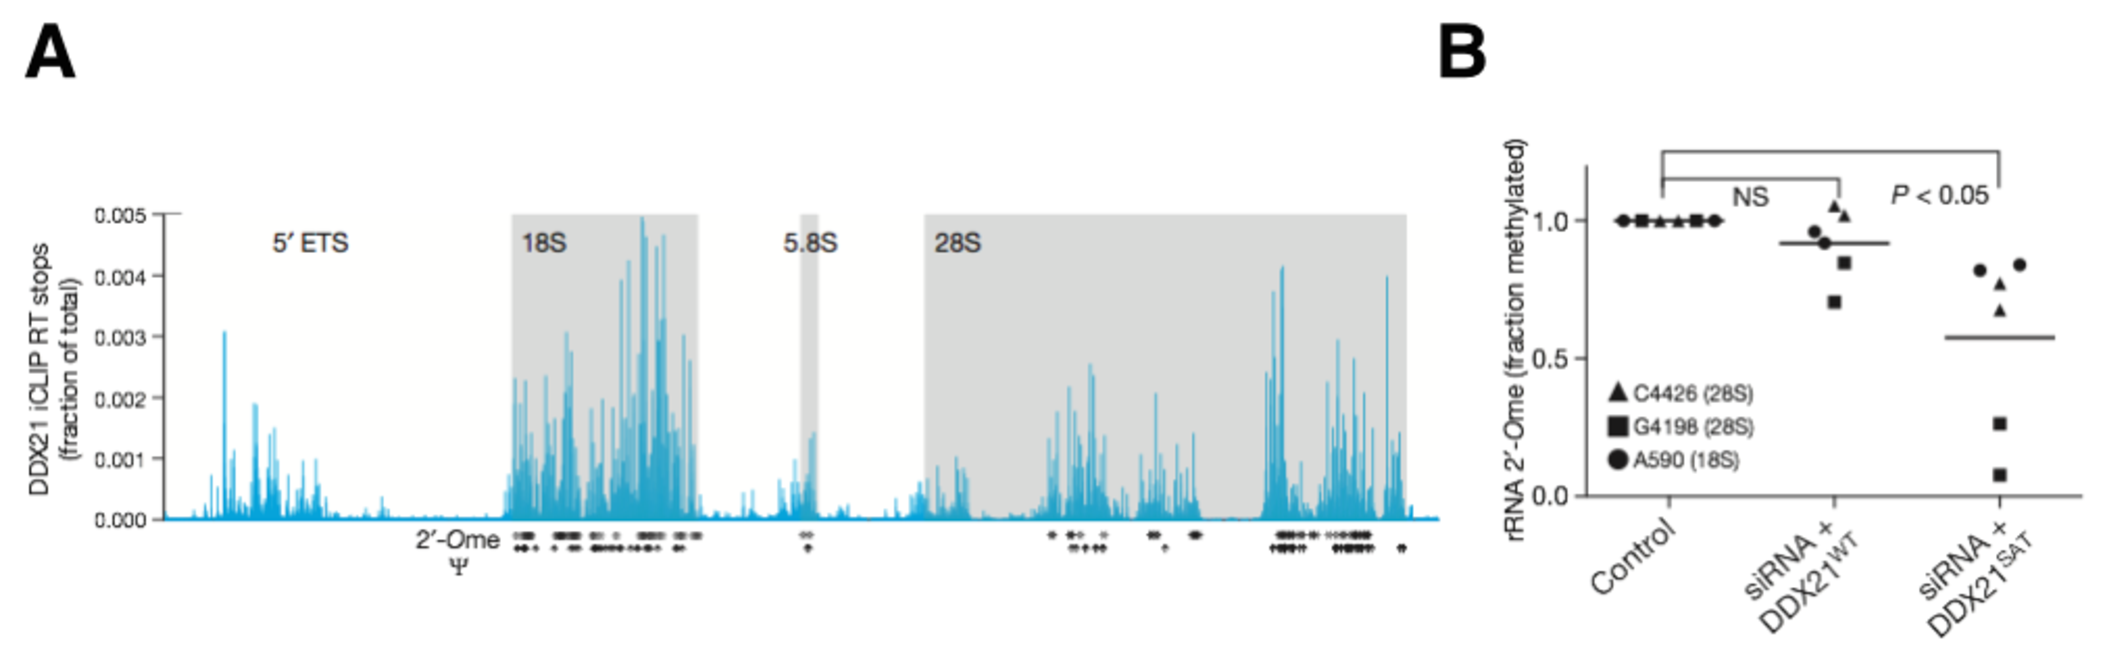
\includegraphics[width=150mm,scale=0.5]{Figures/Fig18}
\caption{The rRNA binding profile of DDX21.}
\label{fig:Fig18}
\end{figure*}

This can be tested by assaying specific rRNA modification expected to be controlled by DDX21-dependent snoRNP function. In turn, we knocked-down DDX21 via siRNA-mediated inhibition and assayed for 2\'-O-methylation (2\'-Ome) using site-directed cleavage of rRNA by RNaseH. Naive topological analysis suggested overlap in DDX21 binding to rRNA and 2\'-Ome sites. We assayed resume of 2\'-Ome in siRNA-treated cells using wild-type DDX21 ask well as a DDX21 mutation that lacks the ATPase domain. As expected, the DDX21 mutant failed to rescue the 2\'-Ome defect. 

The study highlighted a few reasonable points about these experiments and use of the pipeline: (1) Analyzing oft ignored classes of non-coding RNAs, such as snoRNAs, can reveal novel, testable hypothesis. (2) By producing data types that are easily comparable, the comparative analysis between different proteins or experiments is possible and useful. (3) CLIP-derived hypotheses should be tested using functional studies and experiment. In sum, it appeared that the assay and pipeline can reveal biological insights, which admit well to experimental validation.

\subsection{Summary}

The strategy we developed (termed FAST-iCLIP) incorporates a protocol that reduces experimental time by 50\% with a computational pipeline that produces standardized data sets across protein coding, noncoding, and user-definable nonhuman transcriptomes. As sequencing continues to reveal novel noncoding RNA classes and further characterize microbial biodiversity, FAST-iCLIP can scale beyond the current human- and protein centric scope of CLIP study investigation.
